%\usepackage{chancery}

%\usepackage{tikz}
\usetikzlibrary{
   arrows.meta,
   backgrounds,
   calc,
   decorations.pathmorphing,
   decorations.text,
   shapes.geometric,
}

\resizebox{.99\textwidth}{!}{%

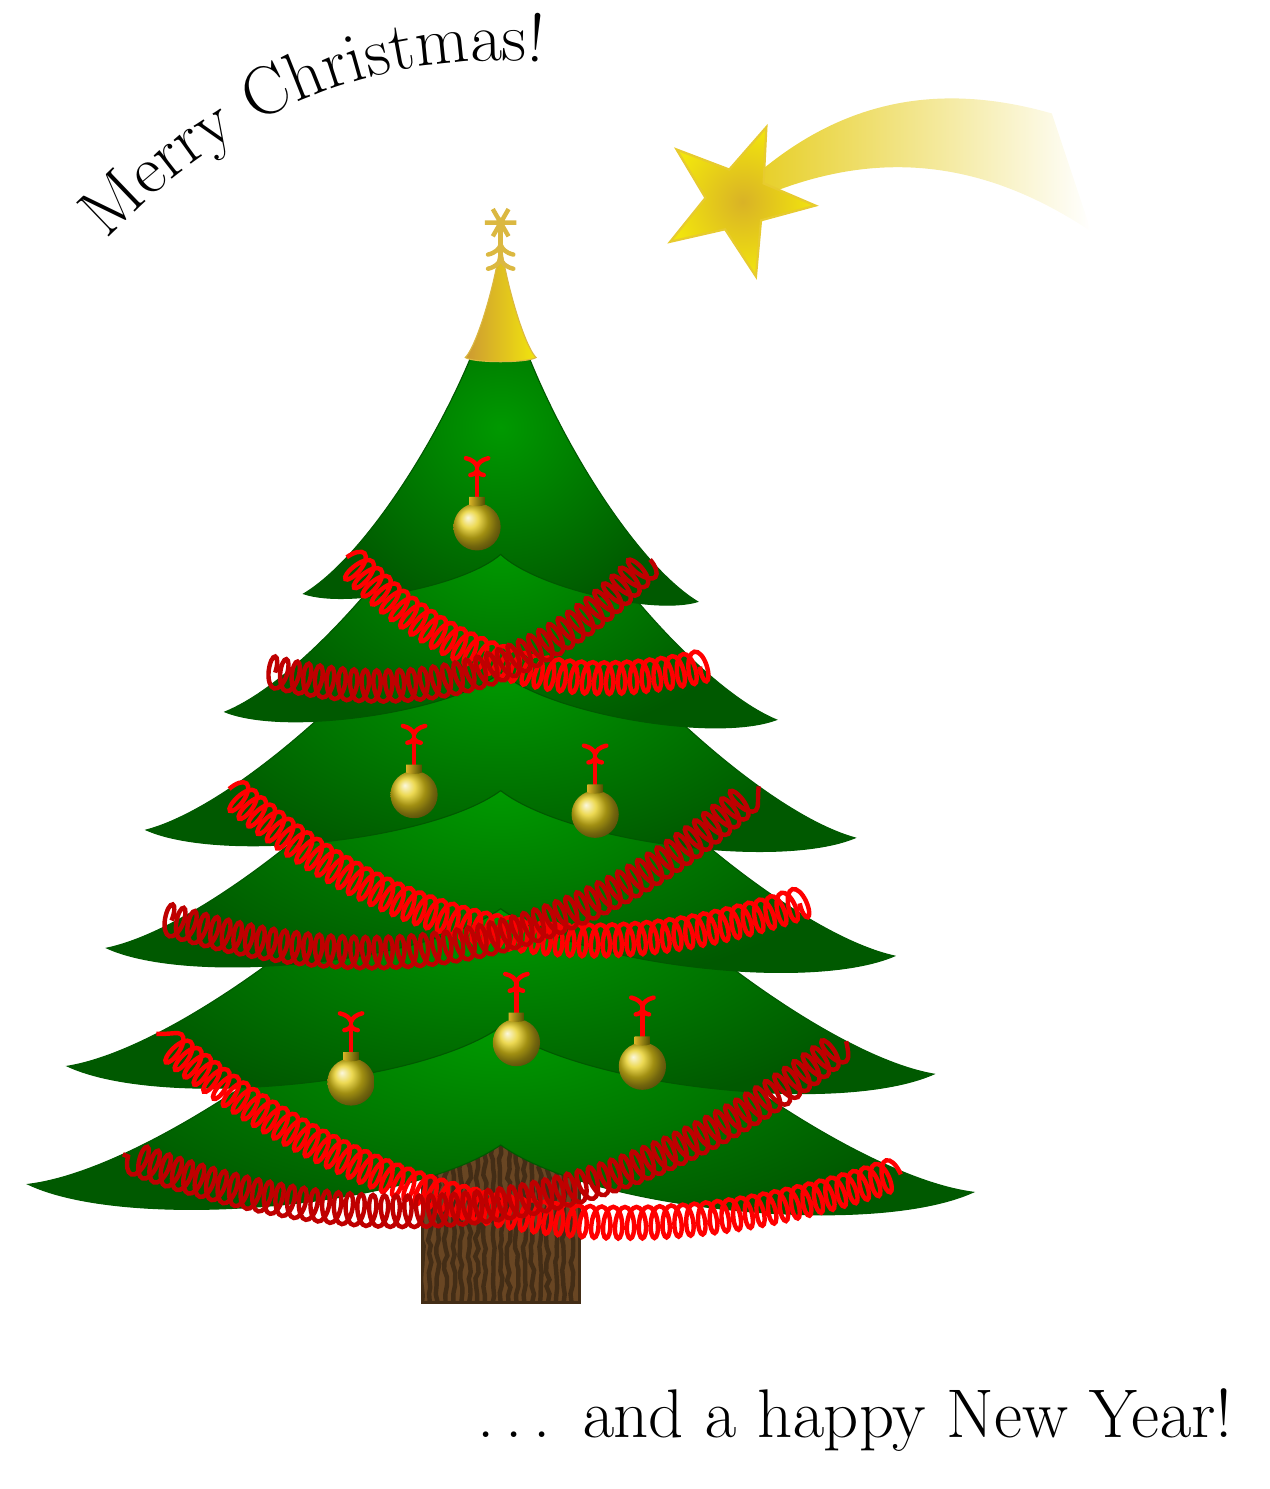
\begin{tikzpicture}[
   bauble/.pic = {
      \shade [ball color = yellow!60!brown]
         (0,-0.9) circle [radius = 0.3];
      \draw [
         ultra thick,
         red,
         -{>[scale=0.6]<[scale=0.9]},
      ] (0,-0.6) -- (0,0);
      \shade [
         left color = yellow!40!brown,
         right color = yellow!30!black,
      ]
         (-0.1,-0.62) to[bend right, looseness = 0.6]
         (0.1,-0.62) -- ++(0,0.1) -| cycle;
   },
]

   % Star
   \node (Stern) [
      star,
      star point height = 6mm,
      minimum size = 20mm,
      thick,
      draw = yellow!60!brown,
      inner color = yellow!40!brown,
      outer color = yellow!80!brown,
      rotate = 50,
   ] at (3,14) {};
   \begin{scope}[on background layer]
      \shade [
         left color = yellow!60!brown,
         right color = white,
      ]
         ($(Stern.center)-(0,0.1)$) -- ($(Stern.center)+(0,0.1)$)
         to[bend left] ++(4,1) -- ++(0.5,-1.5)
         to[bend right] cycle;
   \end{scope}
   % Trunk
   \begin{scope}
      \filldraw [
         fill = brown!55!black,
         draw = brown!35!black,
         thick,
      ] (-1,0) rectangle (1,2);
      \clip (-1,0) rectangle (1,2);
      \foreach \x in {-1,-0.9,...,1}
         \draw [
            brown!35!black,
            ultra thick,
            decoration = {
               random steps,
               segment length = 1mm,
               amplitude = 0.25mm
            }, decorate
         ] (\x,0) -- ++(0,2);
   \end{scope}
   % Branches
   \foreach \b/\y [count = \n]
   in {6/2, 5.5/3.5, 5/5, 4.5/6.5, 3.5/8, 2.5/9.5}
      \shadedraw [
         outer color = green!35!black,
         inner color = green!60!black,
         draw = green!35!black,
         looseness = 0.6,
      ]
         (-\b,\y-0.5) coordinate (L-\n)
         to [bend right] coordinate [midway] (LM-\n)
         (0,\y) coordinate (M-\n)
         to [bend right] coordinate [midway] (RM-\n)
         (\b,\y-0.6) coordinate (R-\n)
         to [bend left] coordinate [pos = 0.2 + 0.05*rand] (RS-\n)
         (0,\y+4) coordinate (S-\n)
         to [bend left] coordinate [pos = 0.8 + 0.05*rand] (LS-\n)
         cycle;
   % Top
   \shadedraw [
      left color = yellow!20!brown,
      right color = yellow!80!brown,
      draw = yellow!40!brown,
      looseness = 0.4,
   ] ($(S-6)-(0.45,1.5)$)
      to [bend right] ++(0.9,0) 
      to [bend left] ($(S-6)+(0,0.25)$)
      to [bend left] cycle;
   \draw [
      draw = yellow!40!brown,
      ultra thick,
      >>-{Rays[n = 6, width = 4mm, length = 4mm]},
      line cap = round,
   ] ($(S-6)+(0,-0.4)$) -- ++(0,0.8);
   % Decoration
   \begin{scope}[
      ultra thick,
      decoration = {
         coil,
         aspect = 0.4,
         amplitude = 2mm,
         segment length = 1.5mm,
      },
   ]
      \draw [red, decorate, bend right]
         (LS-6) to (RS-5)
         (LS-4) to (RS-3)
         (LS-2) to (RS-1);
      \draw [red!75!black, decorate, bend left]
         (RS-6) to (LS-5)
         (RS-4) to (LS-3)
         (RS-2) to (LS-1);
   \end{scope}
   % Baubles
   \path
      ($(S-6)-(0.3,2.75)$) pic {bauble}
      ($(S-4)-(1.1,3.15)$) pic {bauble}
      ($(S-4)+(1.2,-3.4)$) pic {bauble}
      ($(S-2)-(1.9,3.8)$)  pic {bauble}
      ($(S-2)+(0.2,-3.3)$) pic {bauble}
      ($(S-2)+(1.8,-3.6)$) pic {bauble};
   % Texts
   \path [
      decoration = {
         text along path,
         text = {|\Huge|Merry Christmas!},
         text align = left,
      }, decorate,
   ] (-5,13.5) to[bend left] ++(7,2);
   \node [
      font = \Huge,
   ] at (4.5,-1.5) {\dots\ and a happy New Year!};
   % Show tree coordinates
%   \foreach \n in {1,...,6}
%      \filldraw [
%         draw = white,
%         thick,
%         every node/.style = {
%            above = 1pt,
%            font = \sffamily\scriptsize,
%            fill = white,
%            inner sep = 1pt,
%         },
%         every circle/.style = {
%            radius = 0.6mm
%         },
%      ]
%         (L-\n)  circle node {L-\n}
%         (LM-\n) circle node {LM-\n}
%         (M-\n)  circle node {M-\n}
%         (RM-\n) circle node {RM-\n}
%         (R-\n)  circle node {R-\n}
%         (RS-\n) circle node {RS-\n}
%         (S-\n)  circle node {S-\n}
%         (LS-\n) circle node {LS-\n};
\end{tikzpicture}

}  %% resizebox END